\section{Big Data and Distributed Systems}

We start from the problem that created NoSQL databases: data that no longer fits the classical single-server approach.

\subsection{What is Big Data}
\begin{definition}[Big Data]
Any problem characteristic that represents a challenge to process it with traditional applications. It involves data whose volume, diversity and complexity require new techniques, algorithms and analyses to fetch, store and elaborate them.
\end{definition}

Big Data comes from social networks, scientific instruments and sensors, mobile devices, transactions and genomics. It was first described by the \g{5 Vs}:
\begin{itemize}
  \item \g{Volume}: huge amount of data.
  \item \g{Velocity}: data is accumulated at high speed.
  \item \g{Variety}: different formats from various sources.
  \item \g{Veracity}: inconsistencies and uncertainty in the data.
  \item \g{Value}: the data must be useful.
\end{itemize}
The list later grew to 10 Vs (adding \s{validity}, \s{variability}, \s{venue}, \s{vocabulary}, \s{vagueness}) and to 42 Vs in 2017.

\begin{remark}
The project dataset must be real, at least 50/100\,MB, and must show at least one between \s{variety} (multiple sources or formats) and \s{velocity/variability} (data that loses importance because new data arrives).
\end{remark}

Working with Big Data means dealing with acquisition, storage, computing infrastructure, querying, analytics, visualization, security and privacy. Classical algorithms cannot be applied directly, so we need new technologies for both storage and computation.

\subsection{Scale-up vs scale-out}
\begin{itemize}
  \item \g{Scale-up} (vertical): move to a bigger machine. It has a single point of failure, requires outages during migration, and a bigger machine usually costs more than several small ones.
  \item \g{Scale-out} (horizontal): use a \g{cluster} of small machines and add or remove nodes following the load. Costs stay reasonable, but we must manage distributed data.
\end{itemize}

In a distributed system one machine cannot store or process all the data, so data is spread over the nodes. For the user it must not matter which machine runs an operation, or whether it runs twice because of a failure or a slow (\s{straggler}) node. The crucial point is \g{data locality}: we move the computation to the data and avoid transfers between machines as much as possible. Typically a distributed file system splits each file into \g{chunks} and stores each chunk on several nodes.

\subsection{MapReduce, Hadoop and Spark}
\g{MapReduce} (Google, 2004) is a parallel programming model based on divide and conquer:
\begin{enumerate}
  \item \g{Map}: each node processes its local chunk and emits key-value pairs.
  \item \g{Shuffle}: pairs with the same key are sent to the same node. Only the necessary data moves on the network.
  \item \g{Reduce}: values of the same key are combined.
\end{enumerate}

\begin{example}[WordCount]
Map emits \texttt{(word, 1)} for each word of each chunk, shuffle groups equal words, and reduce sums the values, producing \texttt{(word, count)}.
\end{example}

\g{Apache Hadoop} is the first widely used open-source framework. Its modules are \s{Hadoop Common}, \g{HDFS} (fault-tolerant distributed file system for big files on low-cost hardware, efficient for reads and appends), \g{YARN} (job scheduling and resource management) and \s{Hadoop MapReduce}. It is optimized for \s{one-pass batch} processing on disk, so it is slow for iterative or online computation.

\g{Apache Spark} solves this with \g{in-memory cluster computing}: datasets are cached in memory across iterations. A \g{driver} program runs the main function and sends tasks to the \g{executors}, which run them in parallel. The main abstraction is the \g{RDD} (Resilient Distributed Dataset), a fault-tolerant partitioned collection that can be rebuilt if a portion is lost. DataFrames and Datasets are higher-level abstractions on top of RDDs. Spark is independent of the storage system and reads and writes through connectors.

\section{The Database Revolutions}

The history explains why each model exists: every revolution answers a limit of the previous one.

\subsection{From navigational to relational}
The first electronic databases (around 1960) were \g{OLTP} systems (On-Line Transaction Processing) based on \g{ISAM} (Indexed Sequential Access Method). Each one was built for a specific application, so \g{DBMSs} were introduced: a layer separating database logic from application logic, based on a \g{schema} and on \g{access paths}.

The first DBMSs used \g{navigational models}: \s{hierarchical} (a tree, one parent per record) and \s{network} (a graph, many parents). They supported only queries anticipated at design time, made it hard to add new data, and required hard-coded analytics.

In 1970 \g{Edgar Codd} proposed the \g{relational model}, based on:
\begin{itemize}
  \item \g{tuples} (rows) and \g{relations} (tables), where operations on relations return relations;
  \item \g{constraints}: primary key, foreign key, unique key, plus constraints on values;
  \item \g{normal forms}: in third normal form non-key attributes depend on ``the key, the whole key, and nothing but the key''.
\end{itemize}
Concurrent changes are handled through \g{ACID transactions} (\cref{sec:acid}). SQL was born with IBM System R (1974) and became the standard by the mid-1980s, and client-server architectures then separated the database server from the application.

\subsection{Impedance mismatch and ORM}
Object-oriented programs do not map directly onto tables: this is the \g{object-relational impedance mismatch}. \s{OODBMSs} tried to store objects directly but were not widely adopted. \g{ORM} frameworks (e.g.\ Hibernate) instead map table to class, column to field, row to object and relationship to composition or aggregation.

\begin{remark}
Document databases reduce this mismatch in a different way: a document is already close to an object, with nested fields and arrays.
\end{remark}

\subsection{Web-scale applications and NoSQL}
Around 2005 \g{massive web-scale applications} (Google, Amazon, Facebook, \dots) needed large volumes of reads and writes, low latency, high availability and fault tolerance. Relational systems struggle here: vertical scaling is costly and limited, deployment on many servers is hard, and ACID transactions across servers are expensive. The new requirements were \g{scalability}, \g{flexibility}, \g{availability} and \g{low cost}.

\g{NoSQL} (\s{Not Only SQL}) is a set of data models and software meeting these requirements, often open source and often without full ACID support. \g{NewSQL} systems keep much of the relational model while changing the underlying technology. Cloud SQL services offer scalable relational databases pay-per-use, at the price of less flexibility and possible privacy concerns.

\section{ACID, CAP and BASE}\label{sec:acid}

Every database choice in the project is a trade-off between consistency, availability and latency, so this is the theoretical basis for all the following sections.

\subsection{Replication and its cost}
A DBMS must ensure \g{persistence}, \g{integrity} and \g{availability} of data. To be available despite failures, data is \g{replicated} on multiple servers, but then copies must be kept aligned. There are two extremes:
\begin{itemize}
  \item \g{Two-phase commit}: a write is complete only when all the replicas have acknowledged it. Data is consistent, but the write is slower and queries on that data are blocked meanwhile. The two-phase commit is itself a transaction.
  \item \g{Eventual consistency}: control returns after the write on the primary and a background process propagates it. Responses are fast, but for a while a replica can return an old value.
\end{itemize}

\subsection{ACID transactions}
\begin{definition}[Transaction, Jim Gray]
A transformation of state which has the properties of atomicity (all or nothing), durability (effects survive failures) and consistency (a correct transformation).
\end{definition}
\begin{itemize}
  \item \g{Atomic}: all the statements are applied, or none.
  \item \g{Consistent}: the database is in a consistent state before and after.
  \item \g{Isolated}: a transaction does not see the effects of other in-progress transactions.
  \item \g{Durable}: once saved, changes persist even after an OS or hardware failure.
\end{itemize}

ACID can be \s{too much} when response time matters more than perfectly aligned copies. Amazon estimated about 1\% fewer sales for each extra tenth of a second, and Google a 20\% loss of requests for an extra half second.

\subsection{The CAP theorem}
\begin{theorem}[CAP, Brewer]
A distributed database cannot ensure at the same time more than two of:
\begin{itemize}
  \item \g{Consistency} (C): consistent copies of data on different servers;
  \item \g{Availability} (A): a response to any query;
  \item \g{Partition protection} (P): failures of nodes or connections do not impact the system as a whole.
\end{itemize}
\end{theorem}

\begin{center}
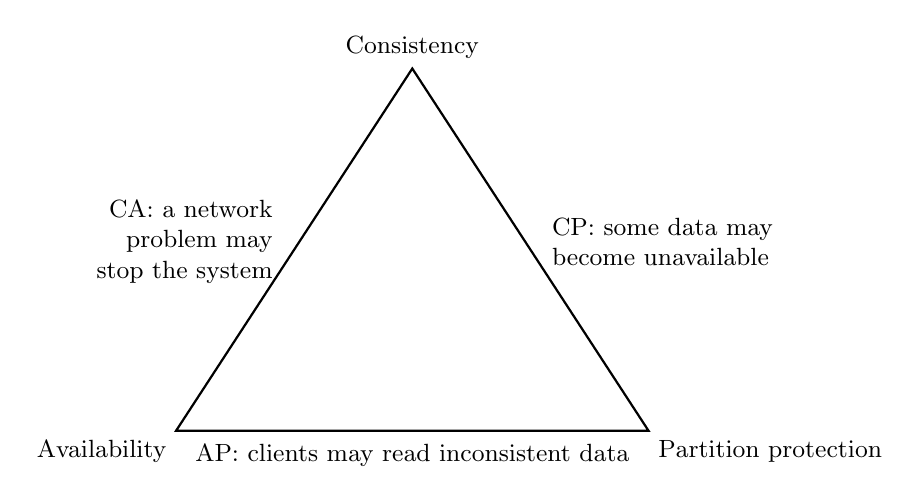
\begin{tikzpicture}[every node/.style={font=\small}]
  \draw[thick] (0,0) -- (6,0) -- (3,4.6) -- cycle;
  \node[above] at (3,4.6) {\g{C}onsistency};
  \node[below left] at (0,0) {\g{A}vailability};
  \node[below right] at (6,0) {\g{P}artition protection};
  \node[left, align=right] at (1.35,2.4) {CA: a network\\problem may\\stop the system};
  \node[right, align=left] at (4.65,2.4) {CP: some data may\\become unavailable};
  \node[below] at (3,-0.05) {AP: clients may read inconsistent data};
\end{tikzpicture}
\end{center}

\begin{table}[h]
\centering\small
\begin{tabular}{p{1cm}p{5.7cm}p{6.2cm}}
\toprule
\textbf{Type} & \textbf{During a network partition} & \textbf{Typical use} \\
\midrule
CA & all operations are blocked until it is resolved & single-site or tightly coupled systems where partitions are rare \\
AP & all operations are allowed, synchronization is suspended, reads may be stale; replicas realign afterwards & shopping carts, news, social networks \\
CP & only the majority partition keeps working, the minority is blocked & banking, ATMs, systems that accept longer response times \\
\bottomrule
\end{tabular}
\end{table}

\begin{remark}
When a partition actually happens, the administrator has only two choices: show each user a possibly different view (AP), or shut down one partition (CP). The AC side is not allowed in this case. In a real cluster partitions must be tolerated, so the actual decision is between C and A.
\end{remark}

\subsection{BASE and eventual consistency}
NoSQL databases often follow \g{BASE} instead of ACID:
\begin{itemize}
  \item \g{Basically Available}: partial failures are handled to keep the service available, often through replication.
  \item \g{Soft state}: data on a node may change because of eventual consistency, even without user writes.
  \item \g{Eventually consistent}: at some point in the future all nodes converge to a consistent state.
\end{itemize}

Eventual consistency distributes over time the latency of synchronization. There are several levels of guarantee:
\begin{itemize}
  \item \g{Read-your-writes}: after updating a record, a user always reads the updated value.
  \item \g{Session}: read-your-writes, but only within one session.
  \item \g{Monotonic read}: after seeing a value, a user never sees an earlier version of it.
  \item \g{Monotonic write}: the updates of a user are executed in the order they were issued.
  \item \g{Causal}: operations with a causal dependency are seen in that order, while unrelated ones can appear in any order.
\end{itemize}

\begin{example}[Causal vs monotonic write]
Pietro writes a post, and Mike and Pippo reply independently. Both replies are causally related to the post, but not to each other: causal consistency requires them to appear after the post, in any relative order. If Pippo instead replies to Mike, Pippo's post must also follow Mike's. Monotonic write only orders the updates of the \s{same} user.
\end{example}
